% !TEX encoding = UTF-8
% !TEX TS-program = pdflatex
% !TEX root = ../tesi.tex

%**************************************************************
\chapter{Introduzione}
\label{cap:introduzione}
%**************************************************************

% Introduzione al contesto applicativo.\\

% \noindent Esempio di utilizzo di un termine nel glossario \\
% \gls{api}. \\

% \noindent Esempio di citazione in linea \\
% \cite{site:agile-manifesto}. \\

% \noindent Esempio di citazione nel pie' di pagina \\
% citazione\footcite{womak:lean-thinking} \\

%**************************************************************
\section{L'azienda}

Sync Lab nasce a Napoli nel 2002 come software house ed è rapidamente cresciuta nel
mercato dell’Information and Comunications Tecnology (ICT) G . 
\\\\
A seguito di una
maturazione delle competenze tecnologiche, metodologiche ed applicative nel dominio
del software, l’azienda è riuscita rapidamente a trasformarsi in System Integrator con-
quistando significative fette di mercato nei settori mobile, videosorveglianza e sicurezza
delle infrastrutture informatiche aziendali. 
\\\\
Attualmente, Sync Lab ha più di 150 clienti
diretti e finali, con un organico aziendale di 300 dipendenti distribuiti tra le 6 sedi
dislocate in tutta Italia.
Sync Lab si pone come obiettivo principale quello di supportare il cliente nella realizza-
zione, messa in opera e governance di soluzione IT, sia dal punto di vista tecnologico,
sia nel governo del cambiamento organizzativo.

\begin{figure}[!h]
    \centering
    
\includegraphics[height=2.5cm]{logo-synclab}
\end{figure}

%**************************************************************
\section{Scelta dell'azienda}

Sono venuto a conoscenza dell'azienda Sync Lab grazie al progetto d'ingegneria del
software, dove l'azienda è stata la proponente del mio progetto.
\\\\
Sono venuto a conoscenza del progetto di stage di Sync Lab grazie all'evento stage-it 2022. 
L’evento promosso da Assindustria Venetocentro in collaborazione con l’Università 
di Padova per favorire l’incontro tra aziende con progetti innovativi in ambito IT e 
studenti dei corsi di laurea in Informatica, Ingegneria informatica e Statistica.
\\\\


%**************************************************************
\section{Introduzione al progetto}

Lo scopo del progetto di stage consiste nell'effettuare la migrazione di un servizio di
API REST lato back-end realizzato da un precedente studente tirocinante con il framework
Spring in un servizio di API REST lato back-end realizzato con un diverso framework, chiamato
NestJS. La migrazione viene fatta per effettuare un'analisi comparativa tra i due servizi, in
modo da valutarne le caratteristiche e decidere quale dei due meglio si adatta alle esigenze
del progetto.
\\\\
Il progetto consiste nella realizzazione di una webapp che si occupa di gestire un sistema
di controllo parcheggi auto. Il sistema va ad interrogare una base di dati contenente
l'informazione inerente allo stato di alcuni sensori di parcheggio fornendo la visualizzazione
dei posti liberi/occupati all'interno di una mappa.
\\\\
L'idea del progetto consiste nel agevolare il client dell'applicativo, in quanto può venire a 
conoscenza della disponibilità di un parcheggio prima di entrarci, evitando quindi
spostamenti inutili nel caso il parcheggio sia pieno.
\\\\
E' prevista poi la realizzazione di una sezione dedicata ai manutentori, per verificare lo 
stato dei sensori, facilitando quindi il processo di manutenzione.
\\\\
Il progetto è formato da una parte di front-end, realizzata con il framework Angular e una 
parte di back-end che consiste di un servizio di REST API, realizzato in due versioni: una 
con il framework Spring e una con il framework NestJS.

\begin{figure}[!h]
    \centering
    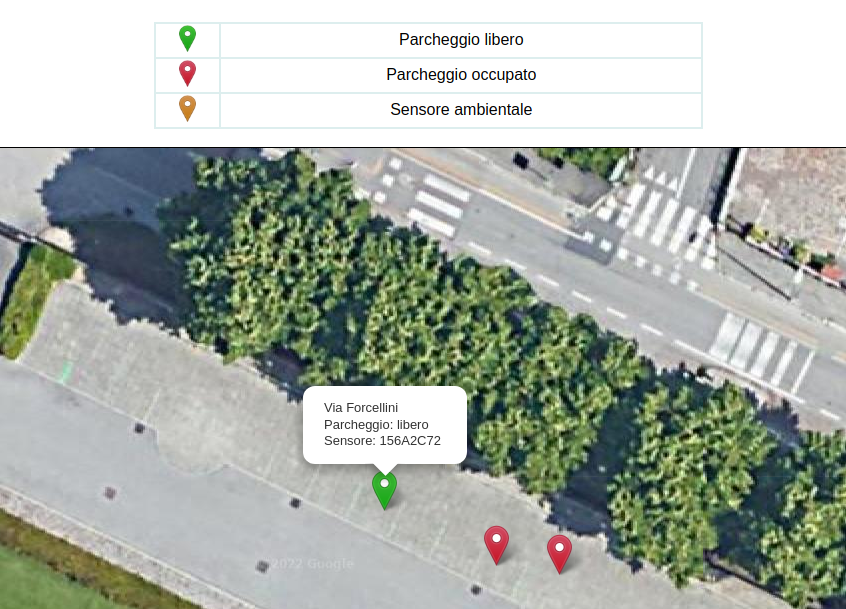
\includegraphics[height=9cm]{front-end-smart-parking}
\end{figure}

%**************************************************************
\section{Problematiche riscontrate}

Problematiche dovute alla mancanza di conoscenza delle tecnologie:
\begin{itemize}
    \item Architettura a microservizi: avevo solo una conoscenza basilare
          della tecnologia, grazie al corso d'ingegneria del software ma non
          sufficiente per sviluppare il progetto.
    \item Framework Spring: la conoscenza di questo framework era completamente assente
        ed era importante conoscerlo per poter comprendere con chiarezza il software esistente
        di cui doveva essere effettuata la migrazione.
    \item Framework Node.js e NestJS: la conoscenza di questi due framework era completamente
        assente era di fondamentale importanza conoscerli per poter implementare il servizio
        di REST API lato back-end richiesto.
\end{itemize}
\leavevmode\newline
Problematiche a livello architetturale:
\begin{itemize}
    \item La quantità di REST API da migrare era troppo elevata per il tempo a disposizione.
    \item Il database in uso si è rivelato avere dei problemi, quindi è stato necessario ristrutturarlo.
\end{itemize}

%**************************************************************
\section{Soluzione scelta}

E' stato scelto di sviluppare con un architettura di tipo layered architecture. Questo è uno
degli stili architetturali più utilizzati quando si sviluppa un monolite. L'idea dietro a 
questa architettura è che i moduli con funzionalità simili sono organizzati in livelli
orizzontali. Quindi ogni livello svolge uno specifico ruolo nell'applicazione.
\\\\
La layered architecture astrae la visione del sistema nel suo insieme, fornendo dettagli 
sufficienti per comprendere ruoli e le responsabilità dei singoli livelli e le relazioni
che intercorrono tra loro.
\\\\
La motivazione che ha portato alla scelta di questo stile architetturale è un'analisi fatta
che ha rivelato la layered architecture adattarsi molto bene al servizio di REST API che
si voleva andare a realizzare ed inoltre il fatto
che molti framework per lo sviluppo di applicativi back-end si basano su esso, tra cui
Spring e NestJS, che sono fondati sul pattern controller-service-repository. Un pattern
che sfrutta la layered architecture, creando tre diversi livelli: 
\begin{itemize}
    \item controller: è il livello più alto ed è l'unico responsabile dell'esposizione delle
        funzionalità in modo che possano essere consumate da entità esterne.
    \item service: livello centrale, gestisce tutta la business logic.
    \item repository: livello più basso, è responsabile di salvare e recuperare i dati da un
        sistema di persistenza, come un database.
\end{itemize}
\leavevmode\newline
\\
Questa struttura viene utilizzata per effettuare una buona separazione delle responsabilità.
L'architettura usata da Spring e NestJS ha portato a sceglierli come framework per realizzare
la parte back-end del progetto.
\leavevmode\newline
\begin{figure}[!h]
    \centering
    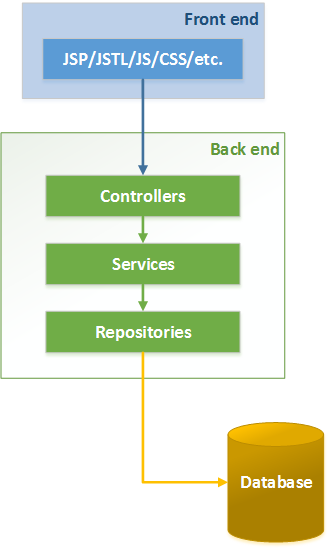
\includegraphics[height=9cm]{controller-service-repository-pattern}
\end{figure}

Non è prevista la creazione di un sistema di autenticazione per l'uso delle API, in quanto 
un altro studente tirocinante si stava occupando della creazione di questa parte.

%**************************************************************
\section{Descrizione del prodotto ottenuto}

Al momento è disponibile un back-end contenente le REST API sviluppate in NestJS, utilizzabile,
in quanto non potendo migrare l'intero set di REST API disponibili in Spring, come preventivato,
sono state sviluppate tutte le REST API più importanti per effettuare le operazioni CRUD più
comuni.
\\\\
Le REST API espongono un'interfaccia compatibile con quello che ormai è uno standard per la
comunicazione con servizi di tipo REST. Ovvero per comunicare con le REST API bisogna fare
delle richieste HTTP a degli specifici endpoint con i seguenti metodi HTTP:
\begin{itemize}
    \item GET: per ottenere delle risorse dal servizio REST
    \item POST: per creare una nuova risorsa nel servizio REST
    \item PUT: per modificare una risorsa nel servizio REST
    \item DELETE: per eliminare una risorsa dal servizio REST
\end{itemize}
\leavevmode\newline
E' presente poi un servizio schedulato che ogni due minuti in maniera autonoma va a fare il polling
da un file XML online, contenente gli stati aggiornati dei sensori. Questo servizio registra poi 
le variazioni, rispetto
al polling precedente, nel servizio di persistenza.
\\\\
Il file XML viene scritto e gestito dai produttori dei sensori di parcheggio, quindi non è compito di questo 
progetto gestirne il funzionamento. Il funzionamento di questo file è comunque abbastanza banale,
in quanto ad ogni variazione di stato il sensore di parcheggio va semplicemente ad aggiornare 
il record a lui associato
all'interno del file.
\\\\

%**************************************************************
\section{Tecnologie utilizzate}

Git
\\
E' uno degli strumenti di controllo di versionamento più utilizzati. Facilita la collaborazione
di più sviluppatori nella realizzazione di un progetto e permette con semplicità di spostarsi
tra varie versioni del software realizzate. Nel progetto è stato utilizzato con il workflow
Gitflow.
\\\\
Visual Studio Code
\\
E' un editor di codice sorgente sviluppato da Microsoft che aiuta molto lo sviluppatore durante la fase
di sviluppo del codice in quanto evidenzia le parole chiave, segnala errori di scrittura, suggerisce
snippet di codice. Possiede una grande libreria di estensioni facilmente installabili, per renderlo
compatibile con praticamente qualsiasi linguaggio di programmazione.
\\\\
Postman
\\
E' un'applicazione che viene utilizzata solitamente per testare API. E' un client HTTP che testa richieste
HTTP, utilizzando una GUI, attraverso la quale otteniamo diversi tipi di risposta in base alle API che 
andiamo ad interrogare.
\\\\
Stoplight
\\
E' una piattaforma per disegnare API. Grazie a questo strumento è possibile documentare in maniera rigorosa
e su uno spazio in cloud un set di API. La piattaforma permette di specificare varie informazioni per ogni
API, tra cui endpoint, parametri in ingresso attesi, possibili risposte con status code associato. Questo
strumento è molto utile per gli sviluppatori front-end che devono chiamare le API di un servizio
back-end, soprattutto grazie alla funzionalità che permette di effettuare il mock della risposta di un'API.
\\\\
TypeScript
\\
E' un superset di JavaScript, che aggiunge tipi, classi, interfacce e moduli opzionali al JavaScript 
tradizionale. Si tratta sostanzialmente di una estensione di JavaScript.
TypeScript è un linguaggio tipizzato, ovvero aggiunge definizioni di tipo statico: i tipi consentono di 
descrivere la forma di un oggetto, documentandolo meglio e consentendo a TypeScript di verificare che 
il codice funzioni correttamente.
\\\\
Node.js
\\
E' un framework per realizzare applicazioni Web in JavaScript, permettendoci di utilizzare questo 
linguaggio, tipicamente utilizzato nella client-side, anche per la scrittura di applicazioni server-side.
La piattaforma è basata sul JavaScript Engine V8, che è il runtime di Google utilizzato anche da Chrome e 
disponibile sulle principali piattaforme, anche se maggiormente performante su sistemi operativi UNIX-like.
\\\\
NestJS
\\
E' un framework per la creazione di applicazioni lato server Node.js efficienti e scalabili. 
Utilizza JavaScript ma è costruito con e supporta completamente TypeScript. Aggiunge un livello di astrazione
al framework Express, che a sua volta aggiunge astrazione al framework Node.js. Di conseguenza NestJS 
utilizza Node.js per eseguire il codice JavaScript prodotto dal codice TypeScript compilato.
\\\\
Spring
\\
Spring è un framework leggero, basato su Java. Questo framework integra soluzioni a vari problemi tecnici
che si presentano con alta frequenza durante lo sviluppo software. Spring si basa su due design pattern
fondamentali che sono l'Inversion of Control e Dependency Injection.
\\\\
PostgreSQL
\\
Chiamato anche Postgres, è un sistema di database relazionale a oggetti (ORDBMS), open source e 
gratuito.
Le principali caratteristiche di Postgres sono affidabilità, integrità dei dati, funzionalità ed estensibilità, 
oltre alla propria community open source che gestisce, aggiorna e sviluppa soluzioni performanti e innovative.
\\\\
Jest
\\
Jest è un framework di unit test sviluppato da Facebook. Focalizzato sulla semplicità, è utilizzabile in qualsiasi
progetto JavaScript. E'uno dei framework di test JavaScript più popolare in questi giorni e la scelta di default 
per alcuni framework come NestJS e React.
\\\\
Winston
\\
% TODO: descrivere winston
\\\\
Npm
\\.
E' uno dei gestori di pacchetti per il linguaggio JavaScript più popolare. E' il gestore di pacchetti predefinito 
per Node.js.

%**************************************************************
\section{Organizzazione del testo}

\begin{description}
    \item[{\hyperref[cap:analisi-requisiti]{Il secondo capitolo}}] descrive l'analisi dei requisiti.
    
    \item[{\hyperref[cap:progettazione]{Il terzo capitolo}}] approfondisce la fase di progettazione.
    
    \item[{\hyperref[cap:ristrutturazione-database]{Il quarto capitolo}}] descrive la fase di ristrutturazione del database.
    
    \item[{\hyperref[cap:verifica-e-validazione]{Il quinto capitolo}}] descrive la fase di verifica e validazione.
    
    \item[{\hyperref[cap:analisi-comparativa]{Il sesto capitolo}}] approfondisce l'analisi comparativa tra la soluzione in Spring e quella in NestJS.
    
    \item[{\hyperref[cap:conclusioni]{Il settimo capitolo}}] presenta le conclusioni finali sul progetto e sull'esperienza di stage.
\end{description}

Riguardo la stesura del testo, relativamente al documento sono state adottate le seguenti convenzioni tipografiche:
\begin{itemize}
	\item gli acronimi, le abbreviazioni e i termini ambigui o di uso non comune menzionati vengono definiti nel glossario, situato alla fine del presente documento;
	\item per la prima occorrenza dei termini riportati nel glossario viene utilizzata la seguente nomenclatura: \emph{parola}\glsfirstoccur;
	% //TODO: valutare se mettere e implementare questo:
    % \item i termini in lingua straniera o facenti parti del gergo tecnico sono evidenziati con il carattere \emph{corsivo}.
\end{itemize}